\section{Attack}\label{sec:attack}

\begin{figure}
    \centering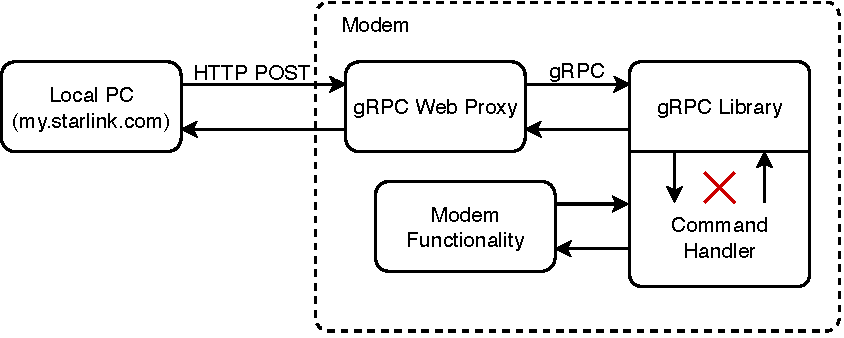
\includegraphics[width=\columnwidth]{img/modem.pdf}
    \caption{Overview of the Starlink modem functionality. gRPC calls are encapsulated within HTTP POST requests by the web interface, which are decoded and processed. Malformed gRPC requests cause the command handler to crash, resulting in the modem no longer being able to respond to commands.}
    \label{fig:modem}
\end{figure}

In this section we explore the underlying architecture of the Starlink modem, and how this opens the system up to denial-of-service attacks.

The user terminal is typically administered via the ``\url{my.starlink.com}'' web interface.
This interface makes calls to the modem over the local network, using the gRPC (Google Remote Procedure Calls) framework for sending remote commands~\cite{gRPC}.
These in turn are encapsulated within HTTP ``POST'' requests, allowing the browser to \textbf{TODO ???}
Although typically sent using the web interface, these gRPC calls can be made on their own from any device or application on the local network \textbf{TODO}.
For instance, the \textit{grpcurl} utility provides a command-line interface for gRPC commands, and can be used to query the modem for available functions~\cite{gRPCurl}.
To make HTTP-encapsulated gRPC requests, tools like \textit{curl} can be used \textbf{TODO cite?} -- however, the encoding of the command needs to be known ahead of time.
This can be extracted using a network monitor such as \textit{Wireshark} \textbf{TODO cite?}.

Although some commands require password authentication, the vast majority do not.
Among these are telemetry and status requests, logging, and commands on the dish itself.
As a result, an adversary on the local network can trivially cause rudimentary denial of service -- for example, by sending the ``stow'' command to rotate the dish away from the sky, leaving it unable to connect to satellites overhead.
By repeatedly sending these commands, service is persistently denied.

When encapsulated within HTTP requests, gRPC commands are very small -- the payload is usually between 2 and 5 bytes.
This gives a sufficiently small command space for effective fuzzing, since we can send commands of the correct format with random contents to see if any are valid.
Through this approach we can find not only valid commands, but also invalid commands that expose corner cases in the command handler, causing unexpected behavior.
One such command is the byte sequence \lstinline{\x00\x00\x00\x00\x03\xea>\x00}, which causes the command handler to crash -- this is shown in Figure~\ref{fig:modem}.
This stops the modem from responding to commands, but does not stop the terminal from functioning, effectively freezing its settings and state until the terminal is rebooted.
A physical power-cycle is required in order to restore functionality.

Appendix~\ref{app:stow-and-kill} contains a shell script to send the malformed command to a user terminal on the local network.
\textbf{TODO maybe picture of error message and/or stowed dish?}